\documentclass{sigchi}

% Use this section to set the ACM copyright statement (e.g. for
% preprints).  Consult the conference website for the camera-ready
% copyright statement.

% Copyright
\CopyrightYear{2016}
%\setcopyright{acmcopyright}
\setcopyright{acmlicensed}
%\setcopyright{rightsretained}
%\setcopyright{usgov}
%\setcopyright{usgovmixed}
%\setcopyright{cagov}
%\setcopyright{cagovmixed}
% DOI
\doi{http://dx.doi.org/10.475/123_4}
% ISBN
\isbn{123-4567-24-567/08/06}
%Conference
\conferenceinfo{CHI'16,}{May 07--12, 2016, San Jose, CA, USA}
%Price
\acmPrice{\$15.00}

% Use this command to override the default ACM copyright statement
% (e.g. for preprints).  Consult the conference website for the
% camera-ready copyright statement.

%% HOW TO OVERRIDE THE DEFAULT COPYRIGHT STRIP --
%% Please note you need to make sure the copy for your specific
%% license is used here!
% \toappear{
% Permission to make digital or hard copies of all or part of this work
% for personal or classroom use is granted without fee provided that
% copies are not made or distributed for profit or commercial advantage
% and that copies bear this notice and the full citation on the first
% page. Copyrights for components of this work owned by others than ACM
% must be honored. Abstracting with credit is permitted. To copy
% otherwise, or republish, to post on servers or to redistribute to
% lists, requires prior specific permission and/or a fee. Request
% permissions from \href{mailto:Permissions@acm.org}{Permissions@acm.org}. \\
% \emph{CHI '16},  May 07--12, 2016, San Jose, CA, USA \\
% ACM xxx-x-xxxx-xxxx-x/xx/xx\ldots \$15.00 \\
% DOI: \url{http://dx.doi.org/xx.xxxx/xxxxxxx.xxxxxxx}
% }

% Arabic page numbers for submission.  Remove this line to eliminate
% page numbers for the camera ready copy
% \pagenumbering{arabic}

% Load basic packages
\usepackage{balance}       % to better equalize the last page
\usepackage{graphics}      % for EPS, load graphicx instead 
\usepackage[T1]{fontenc}   % for umlauts and other diaeresis
\usepackage{txfonts}
\usepackage{mathptmx}
\usepackage[pdflang={en-US},pdftex]{hyperref}
\usepackage{color}
\usepackage{booktabs}
\usepackage{textcomp}

% Some optional stuff you might like/need.
\usepackage{microtype}        % Improved Tracking and Kerning
% \usepackage[all]{hypcap}    % Fixes bug in hyperref caption linking
\usepackage{ccicons}          % Cite your images correctly!
% \usepackage[utf8]{inputenc} % for a UTF8 editor only

% If you want to use todo notes, marginpars etc. during creation of
% your draft document, you have to enable the "chi_draft" option for
% the document class. To do this, change the very first line to:
% "\documentclass[chi_draft]{sigchi}". You can then place todo notes
% by using the "\todo{...}"  command. Make sure to disable the draft
% option again before submitting your final document.
\usepackage{todonotes}

% Paper metadata (use plain text, for PDF inclusion and later
% re-using, if desired).  Use \emtpyauthor when submitting for review
% so you remain anonymous.
\def\plaintitle{Via: Illuminating Course Choice and Discipline Interactions}
\def\plainauthor{First Author, Second Author, Third Author,
  Fourth Author, Fifth Author, Sixth Author}
\def\emptyauthor{}
\def\plainkeywords{Authors' choice; of terms; separated; by
  semicolons; include commas, within terms only; required.}
\def\plaingeneralterms{Documentation, Standardization}

% llt: Define a global style for URLs, rather that the default one
\makeatletter
\def\url@leostyle{%
  \@ifundefined{selectfont}{
    \def\UrlFont{\sf}
  }{
    \def\UrlFont{\small\bf\ttfamily}
  }}
\makeatother
\urlstyle{leo}

% To make various LaTeX processors do the right thing with page size.
\def\pprw{8.5in}
\def\pprh{11in}
\special{papersize=\pprw,\pprh}
\setlength{\paperwidth}{\pprw}
\setlength{\paperheight}{\pprh}
\setlength{\pdfpagewidth}{\pprw}
\setlength{\pdfpageheight}{\pprh}

% Make sure hyperref comes last of your loaded packages, to give it a
% fighting chance of not being over-written, since its job is to
% redefine many LaTeX commands.
\definecolor{linkColor}{RGB}{6,125,233}
\hypersetup{%
  pdftitle={\plaintitle},
% Use \plainauthor for final version.
%  pdfauthor={\plainauthor},
  pdfauthor={\emptyauthor},
  pdfkeywords={\plainkeywords},
  pdfdisplaydoctitle=true, % For Accessibility
  bookmarksnumbered,
  pdfstartview={FitH},
  colorlinks,
  citecolor=black,
  filecolor=black,
  linkcolor=black,
  urlcolor=linkColor,
  breaklinks=true,
  hypertexnames=false
}

% create a shortcut to typeset table headings
% \newcommand\tabhead[1]{\small\textbf{#1}}

% End of preamble. Here it comes the document.
\begin{document}

\title{\plaintitle}

\numberofauthors{3}
\author{%
  \alignauthor{Leave Authors Anonymous\\
    \affaddr{for Submission}\\
    \affaddr{City, Country}\\
    \email{e-mail address}}\\
  \alignauthor{Leave Authors Anonymous\\
    \affaddr{for Submission}\\
    \affaddr{City, Country}\\
    \email{e-mail address}}\\
  \alignauthor{Leave Authors Anonymous\\
    \affaddr{for Submission}\\
    \affaddr{City, Country}\\
    \email{e-mail address}}\\
}

\maketitle

\begin{abstract}
Graph theoretic approaches can enable concise observation of how students navigate curricular choices in higher education. We exemplify the approach using 18 years of data describing course enrollments of undergraduates at a large research university. After showing options for how student movement through courses can be mapped onto graphs, we model courses as nodes, and sequential course taking as links. Subsequent examples highlight differences in departmental course sequences, both visually and via modularity computation. We demonstrate the quantification of university wide service course usage with graph based visual and computational approaches. We illustrate the value of graph theoretic approaches for learning scientists, academic administrators, and students.
 \end{abstract}

\category{H.5.m.}{Information Interfaces and Presentation
  (e.g. HCI)}{Miscellaneous}{}{}

\keywords{Course Sequences; Academic Pathways; Graph Visualization}

\section{Introduction}
%%{\color{red}[LOCKED BY ANDREAS]}


%% - What is the problem?
%% - Why is it important?
%% - Why is it hard?
%% - How are current solutions insufficient?
%% - What we do

US higher education is unique in the world in the extent to
which schools expect undergraduates to explore a variety of courses before committing to a field of study. In contrast with virtually all other national postsecondary systems, in which students enter schools and programs with relatively structured curricula, US undergraduates are encouraged to explore a variety of academic options through an iterative course search and selection process. We call a student's
eventual sequence of course elections a {\it pathway}. Pathways are notoriously poorly instrumented for observation by students, educators, administrators or researchers \cite{chambliss2014college}.

While enriching when successful, the contingencies of course elections that accumulate into pathways is poorly understood and are almost always fateful. Ethnographic research suggests that students tend to select courses based on partial, poorly integrated information, in light of logistical constraints and personal preferences that have little directly to do with academics \cite{nathan2006my,rosenbaum2011complexities, rosenbaum2007after}. Absent conscientious design and signposting, students can easily spend time, credit hours, and tuition accumulating courses that do not lead efficiently to majors and completion \cite{bailey2015redesigning}. In addition to students, many other academic stakeholders could benefit from better information about college pathways. The work and priorities of instructors, department chairs, deans, and budget officers are implicated in the relative clarity of pathways and the efficiency with which courses can be sequenced to degree completion. 

%One challenge in mitigating this lack is that each of these
%potential beneficiaries of improvement require investigative equipment
%of different focal lengths.

%Day to day, {\bf academic advisors} on the ground lack tools for
%understanding the characteristics of the numerous majors and programs they are tasked to explain. For example, it is not trivial to identify majors whose requirements have students take courses primarily within one department. Requirement structures for majors such as Computer Science tend to impose this more intradepartmental regime. Other majors, such as History, instead have students consume courses such as economics and political science. Insight into such differences are needed for helping advisers suggest pathways that match their student clients' interests and temperaments.

%{\bf Instructors}, in contrast, require information local to their specific course offerings. Yet they cannot easily answer the question {\it Which majors, and preceding courses feed students into my class?}

%{\bf Department chairs} and {\bf deans} are for different reasons in need of knowing the migration paths of students in and out of departments. Questions such as {\it Does our school offer a rich set of non-major service courses to the rest of the university?}, and {\it are students from across campus uniformly taking advantage of such courses?} are difficult to answer.

%Beyond such specific needs, the myriad of possible pathways through curricula also impedes efforts by university administrators to encourage behaviors that lead to outcomes deemed desirable by their institutions. Such goals might emphasize persistence, intellectual breadth, or readiness for the workplace.

Fortunately the information necessary to observe pathways systematically and at scale is present in all colleges and universities in the form of academic transcripts. Transcripts are the official records documenting courses accumulated by each student as he or she makes academic progress. Yet transcripts typically are housed in tables of databases to which few have access, and in their ``raw'' form exceptionally opaque to interpretation. Most schools have specialized staff who generate specifically requested reports for individuals in high level academic positions\footnote{We acknowledge
here our own version of such a unit, which has provided us with numerous insights into both the information needs, and data semantics at our institution.}, but these personnel typically cannot interact directly with all the parties in need of insight on pathways at varying levels of detail.

%Some universities have created software that surfaces a selection of the needed information broadly to its institution's clients (e.g. \cite{carta}). But these tools focus primarily on the narrower needs of individual students, and therefore lack the ability to provide both overview and detailed insight.

We report here on {\it Via}, an analytic toolkit we have built to observe and understand undergraduate pathways utilizing de-identified transcript data held by a large private research university. Our approach is to provide a zoomable, investigative
instrument for large-scale, qualitative and quantitative
investigations of pathways. Built on graph theory, {\it Via} provides a
visual interface for observing the course sequences embedded in tens
of thousands of transcripts. In addition, {\it Via}'s grounding in graphs
allows us to bring associated mathematical computations to bear on the problem of pathway evolution.

Graph approaches have been applied to a wide variety of other tasks, such as detecting communities \cite{Fortunato2004}, collecting materials for survey articles \cite{ji2015}, the augmentation of collaborative recommendation records \cite{huang2005}, predicting future collaborations between scholars \cite{liben2007}, and suggesting drug interactions \cite{zitnik2018}. Our primary contribution in this paper is to apply graph approaches to the sequencing of academic coursework. Because our analytic strategy relies on data of a sort held by every legally recognized US college and university, it is amenable to application throughout the US postsecondary sector. 

%We explain how the availability of additional data, such as demographic information greatly adds to the results that can be achieved.

In our first approximation here, we convert transcript information describing course enrollments at our case school to directed graphs, with nodes modeling courses, links modeling sequential enrollments, and link weights modeling conditional probabilities of enrolling in a particular course before another one. We partition the graphs by the departments to which each course is officially associated by the university registrar. An existing graphing tool \cite{shannon2003cytoscape} exposes more or less information, depending on chosen zoom levels.

%While the concept is easy to explain, details arise that are not
%immediately obvious. In addition, the most informative mapping from
%enrollments to graphs depends on the questions the graph is intended
%to answer. Resulting mappings can vary widely.

After related work and a brief introduction to our dataset, Section~\ref{sec:methodology} introduces how we construct the node and
edge relationships in the {\em Via} network. Section~\ref{sec:visualization} then demonstrates the visual component of the model.  Section~\ref{sec:analysis} highlights diverse use-cases of our model to address questions of different academic stakeholders: students, instructors, and administrators. This final section demonstrates the wider applicability of our model, by comparing our results against well-studied phenomena in education research.

%\textit{Via} is a tool that enables education researchers to gain insights into how students structure their course decisions. One particularly useful feature of the model for this purpose is the ability to filter by the year a student enrolled in a particular course. This enables us to compare the dynamics of student course decisions across different years.

%has argued that the effect of growing introductory computer science courses has resulted largely as a result of the growing monetary returns that computer science fields offer. Educators fear, however, that the attraction to fields in computer and information science, however, may siphon away students interested in the humanities. Using our graph visualization of academic data we will illustrate that while we can observe an increase in the interest of student enrolling in computer science fields, a number of these courses also serve as popular courses that non-CS majors try out for fun. 


%After related work, and a brief introduction to our dataset,
%Section~\ref{sec:visualization} introduces {\it Via}'s visual
%component. In Section~\ref{sec:mapping} we explain alternative graph
%mapping options, and their implications for questions that can be
%investigated. %Sections~\ref{sec:stud_matrix}/\ref{sec:aggr_matrix}
%detail the necessary processing of enrollment data in preparation to
%their ingestion into the visualization component.





\section{Related Work}

Throughout both the social and physical sciences, graphs are used to visualize, simplify and facilitate computational analysis of complex dynamic systems. Graphs have been applied to model a diverse set of networks such as food chains \cite{Hall1993}, the human genome\cite{Pevzner1989} and ecological systems \cite{Fortin2012}. Within the social science, graphing methods have a long history of being applied to study sociological phenomena \cite{Borgatti2009}. The use of graphs within the social science was particularly spurred on by the insight that human societies could be structured like biological systems. The $19^{th}$ century french philosopher, Emile Durkheim, argued for instance that social regularities could be found in the structure of social environments in which they were embedded \cite{Durkheim1951}. By studying these social regularities it is possible to derive macro-level insights about the structure of human interactions. 

Since the mid 1950s, graphs have been applied to model the flow of information in social and professional networks. As part of the MIT Group Networks Laboratory, Leavitt et al. observed how the structure of inter-personal relationships between groups of coworkers facilitated the spread of information throughout a team of colleagues \cite{Leavitt1951}. More recently, similar methods have been applied to study how workplace professional networks influence the spread of information through company email chains \cite{Fisher2004}. The modeling of knowledge transmission parallels closely how graph theoretic methods have been applied to study social dynamics in the field of education. Citation networks, for instance, are a well researched area of sociology that seek to understand how intellectual advancements spread through academia \cite{Batagelj2003}\cite{Garfield1964}. 


% If individual publications are modeled as nodes in the citation network and edges represent a direct citation of one paper by another it should not be feasible for cycles to exist in the citation network. A similar logic applies to the structuring of course sequences in which cycles are not desirable among introductory classes that are intended to be taken sequentially.

A number of the challenges posed in representing citation networks, such as learning optimal edge weights, are directly applicable to the problem of modeling course sequences. Within citation networks, it is useful to modulate the edge strength between two papers in order to represent the relative influence of a cited paper. Batagelj proposes solutions to this problem by introducing SPC weights on each edge of the network to capture the incoming and outgoing 'flow of information' for a given paper \cite{Batagelj2003}. Hajra et al. also observe an aging phenomena among papers in which the probability that a paper is cited decays with time at an exponential rate proportional to $t^{0.9}$ up to 10 years after its publication date. The $\texit{Via}$ network observes a similar exponential time-dependent probability of two courses being taken sequentially. Moreover, just as citation networks provide a framework for modeling the flow of knowledge within academia, our course sequence network implicitly represents shared and prerequisite knowledge between classes. 

Also analogous to our particular framework is recent work done in the field of representing social connections within massive open online courses (MOOCs). Large online education providers, such as \textit{Coursera}, use thread messaging boards to facilitate collaboration between students. Within these forums any student in a particular course can post a question or remark to start a thread of conversation. The data gathered from these educational messaging boards can enable researchers to study the exchange of information between students \cite{Brinton2016}, the influence of students on others' participation in the course \cite{Sinha2014a} and more general social dynamics of a class.

Sinha et al. for instance model each participant within a particular \textit{Coursera} class as a node and draw a directed edge from a particular thread or sub-thread initiator to any of the people who engaged in that discussion \cite{Sinha2014}. By doing so, the authors are able to represent the flow of topics and engagement within the social dynamics of a certain course. In particular, Sinha et al. were able to analyze measures of degree and betweenness centrality on this model of student engagement, in order to understand the influence of discussion initiators on the overall collaboration of students in the class. The p made clear if we interpret discussion topics as self-contained units of knowledge that are part of a course. 

Similarly to our network construction, Sinha et al. use a gradient coloring of the nodes to indicate a node's relative betweenness centrality. Zhu et al. similarly seek to model the engagement of students in discussion forums on a week-by-week basis using Exponential Graph Models (EGM) \cite{Zhu2016}. The use of EGMs allows the authors to model a student's participation for a given week by incorporating a student's performance for both the previous and subsequent weeks. While inspired by EGMs, our model does not directly include aggregate network statistics in order to compute node and edge properties. Instead, we seek to model the probability of two courses being taken sequentially given data in which the classes may have been taken several time quarters apart. Finally, \textit{NetworkSeer} uses a similar modeling framework as in the previous papers but additionally models individual students' demographic information within the course discussion thread \cite{Wu2016}. Although we do not have direct access to students' demographic data, our model uses a student's final major to study the differences in course-taking behavior between students.

%Our course network takes inspiration from the general form of stochastic EGMs: $$P(Y=y) = \frac{1}{k(\theta)}exp(\theta^Tg(y)),$$ where Y is a random variable representing the network and y is a specific observed network.

The social dynamics of student participation in MOOCs and the spread of knowledge through citation networks are the closest parallel to modeling students' course taking behavior at universities. Courses can be observed as distinct units of information that share overlap and prerequisite knowledge with other courses. Academic publications and forum discussions are similarly self-contained units of knowledge that build upon and interact with other publications and discussion threads, respectively. Given a dearth of direct research in course sequence networks, our \textit{Via} toolkit builds upon the modeling frameworks of citation graphs and MOOC social dynamic networks.

\section{Data}
\label{sec:data}
The dataset we use to build our graph for mapping sequential relationships between classes was obtained directly from the a large American private research university. This dataset contains anonymized class enrollment data for over 52,000 students (both graduates and undergraduates) who were enrolled at the university during any time between Fall 2000 and Fall 2018. Each of the over two million entries in this table includes a unique hash which corresponds to each student, the course in which they enrolled, and the quarter during which they enrolled. Our dataset also contains supplementary information on a student's major during time of enrollment in a course and each student's major upon graduation. Depending on the class of problems of interest, we filter along these additional values.

\subsection{Data Preprocessing}
\label{sec:data_processing}

Data preprocessing involved the parsing of the requisite information made available through the dataset; for each student, all classes are paired with their quarters of enrollment. Student metadata was omitted and only classes in our dataset marked completed (classes not dropped by the student during the quarter) were included.

% \begin{figure}[h!]
% \begin{tcolorbox}
% Abstraction and its relation to programming. Software engineering principles of data abstraction and modularity. Object-oriented pro
% gramming, fundamental data structures (such as stacks, queues, sets) and data-directed design. Recursion and recursive data structures (linked lists, trees, graphs). Introduction to time and space complexity analysis. Uses the programming language C++ covering its
% basic facilities. Prerequisite: 106A or equivalent. Summer quarter enrollment is limited.
% \end{tcolorbox}
% \caption{Course Description for CS106B: Programming Abstraction.}
% \label{course-description}
% \end{figure}

\section{Methodology}
\label{sec:methodology}

\begin{figure}
    \centering
    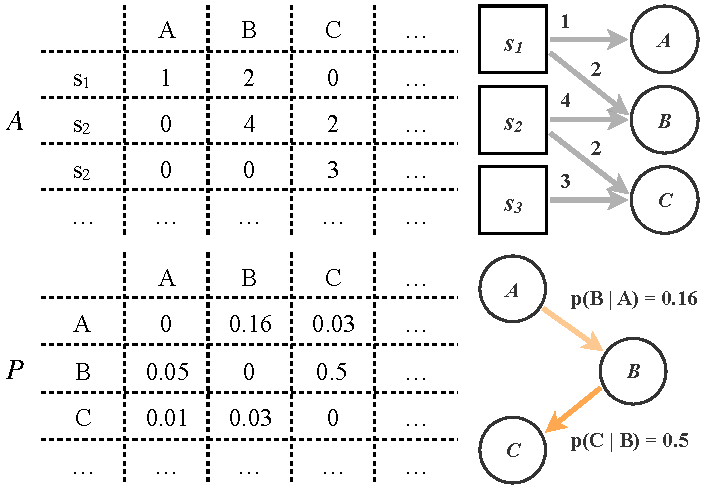
\includegraphics[width=0.75\columnwidth]{final-simple.pdf}
    \caption{A simple visualization of relationships between course \textit{A} and course \textit{B}. }
    \label{fig:simple}
\end{figure}

Our principal objective was to build a powerful, yet interpretable projection model capable of visualizing the sequential relationship of course pairs given a school's enrollment data.

In order to build a succinct representation of these data, we propose a method to compile student-to-course information into what we will call a course-to-course projection model, a network that represents courses as nodes and course relationships as weighted edges. Indeed, we can visualize a simple structure within the graph with the graphic shown in figure 

This model can serve as a toolkit for university stakeholders, allowing them to make more informed decisions about courses. Our graphical framework is built on a flexible projection algorithm that enables the user to adapt the model's visualizations to answer a variety of questions. 

There are two components to the generation of a projection model. The first involves the preparation of a sequence matrix--- the second involves the calculation of the projection itself.

\subsection{Sequence Matrix Generation}
\label{sec:seq_martix}

The Via toolkit receives data that represent student enrollment in courses. The projection algorithm must take a matrix $A$ of shape $(|S|, |C|)$ as input, where $S$ is the set of all students and $C$ is the set of all courses. We can interpret this matrix $A$ as a bipartite multigraph documenting the interaction of student nodes with courses nodes over time. A given entry $A_{ij}$ represents the relative timestep a student $i$ enrolls in some course $j$. For example, an entry $A_{ij} = 1$ signifies that student $i$ enrolled in course $j$ during their first quarter at Stanford. An entry $A_{ij} = 0$ implies that $i$ never enrolled in $j$. This thus implies that each row $A_i$ represents the entire course enrollment history of some student $i$. We generate various forms of matrix $A$ from the raw enrollment data by filtering on different student attributes in order to gain perspectives on different aspects of enrollment behavior. The attribute set we leverage in this analysis are mainly a student's major upon enrollment in a course, a student's final major, and the year in which a course was taken. 

\subsection{Graph Projection}
\label{sec:graph_projection}
%Explain what this graph projection represents
Formally, given a sequence matrix $A$, we generate a final matrix $P$ of shape $(|C|, |C|)$ that can be interpreted as an adjacency matrix for a one-mode projection of the bipartite network that can be generated from the sequence matrix which we explain above. Observe that we do not explicitly create a graph based off of the sequence matrix, rather this matrix serves as an intermediary step in order to generate our final projection graph. A one-mode graph project represents the condensation of a graph by connecting nodes that are of only one type such as courses in our case. The edges in our projection represent a set of conditional probabilities defined between pairs of courses. %TODO: Define what these coditional probabilities mean 
The parameters for these conditional probabilities are fit based on counts determined in the calculation of intermediary matrix $\tilde{P}$ of shape $(|C|, |C|)$ . 

We calculate each entry $\tilde{P}_{ij}$ by accumulating the occurrences of course $i$ taken at some point before course $j$ across all students in set $S$:
\begin{equation}
  \tilde{P}_{ij} = \sum_{s=1}^{|S|} \mathbbm{1}\{A_{si} - A_{sj} \geq 0\}* d(A_{si} - A_{sj})
\end{equation}
where $A_{si} - A_{sj}$ can be interpreted as the academic timestep delta (commonly measured in semesters, or quarters) between a student $s$'s taking course $i$ and course $j$, and $d$ is a function chosen to modulate the signal of the event given the timestep delta if desired. 

The function $d$ may be continuous or discrete.  For example, the
following choice attenuates the relationship between two courses through an
exponential decay:
\begin{equation}
  \tilde{P}_{ij} = \sum_{s=1}^{|S|} \mathbbm{1}\{A_{si} - A_{sj} \geq 0\}* \lambda^{A_{si} - A_{sj}}
\end{equation}
where, $\lambda$ is a constant that controls decay rate. Alternatively, the following choice for $d$ counts a relationship between two courses only when course $j$ immediately follows course $i$. Any
elapsed time in between the two courses severs the relationship:
\begin{equation}
d = \begin{cases} 
      1, & A_{si} - A_{sj} = 1 \\
      0, & A_{si} - A_{sj} > 1 
    \end{cases}
\end{equation}

With $\tilde{P}$, we calculate the final projection matrix $P$. Entry $P_{ij}$ is a conditional probability $p(j|i)$ whose parameters can be computed with the following closed form expression:
\begin{equation}
    P_{ij} = p(j|i) = \frac{\tilde{P}_{ij}}{\sum_{s=1}^{|S|}\mathbbm{1}\{A_{si} > 0\}}
\end{equation}
$P_{ij}$ thus represents the proportion of students who take the course sequence: course $i$ followed by $j$ out of the total number of students who take course $i$ at any point. One may note that this bears a resemblance to a Bayesian Network; however, we make the assumption that the process of transitioning from course node to course node is Markovian in nature. This eases implementation but precludes our model from being a true Bayesian Network due to the emergence of cycles.

Finally, observe that the selection of timestep delta function $d$ greatly influences the relationships expressed by the final projection model. This is by design in order to allow for greater flexibility in the search for solutions to various problem classes. We present results using a discrete function in order to maximize model interpretability.

\section{Graph Visualization}
\label{sec:visualization}

\begin{figure}
    \centering
    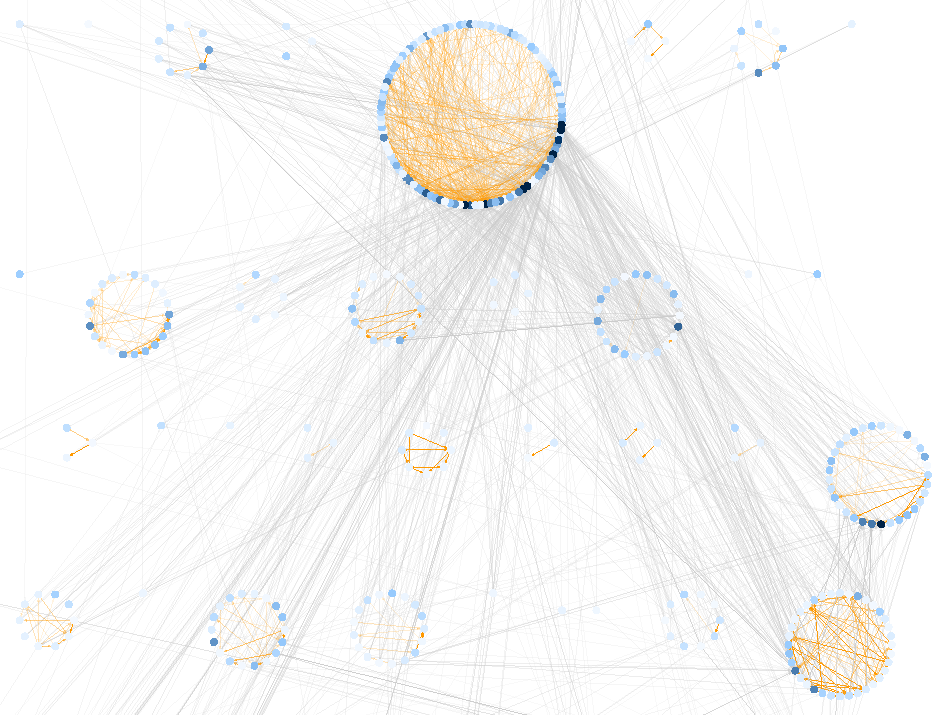
\includegraphics[width=\columnwidth]{final-overview.pdf}
    \caption{An example graph generated using our projection model showcasing behavioral patterns within the CS major. Each ring is comprised of courses offered by different departments.}
    \label{fig:overview}
\end{figure}

We use \textit{Cytoscape}, in order to visualize the  generated network \cite{shannon2003cytoscape}. Cytoscape was developed to model biological systems and interactions between cellular organisms. The visualization infrastructure contains a number of desirable properties for representing our academic pathway data. For one, Cytoscape uses a spring-embedder system for optimally spacing and aggregating nodes, and additionally allows the user to cluster nodes together by attributes \cite{Battista1994}. For our purposes, we aggregate courses within a similar department as ring structures. Moreover, \texit{Cytoscape} allows us to assign unique colorings for both nodes and edges to visualize node and edge-level attributes. In all of the figures below, we color edges between nodes in the same department orange and all edges between courses in different departments grey. We further modulate the thickness of an edge from course \textit{i} to course \textit{j} to represent the relative conditional probability of taking course j after course i. Finally, each node is colored in a blue-gradient representing the probability of a student enrolling in a particular course. A general overview of the \textit{Cytoscape} course sequence visualization is shown in figure \ref{fig:overview}. 

\section{Graph Analysis & Model Applications}
\label{sec:analysis}
In the following sections we will illustrate the applicability of our model to answer a variety of questions posed by university stake-holders. We showcase the use of a graphical representation of our model in order to both visualize general shifts in course enrollments across university departments and to facilitate student, instructor, and administrative decisions at universities. We will use concepts from graph theory in order to bolster qualitative claims that have been posited within education research literature. Our analysis will leverage both the visual and computational power that \textit{Via} provides. 

\subsection{Course Preference Evolution}
\label{sec:course_pref_evolution}

We begin by showing how our model can highlight developments in patterns of course enrollment over a set period of time. The conclusions we derive from our analysis are directly applicable only to the private university from which we acquire our data. However, the manner in which we employ the \textit{Via} toolkit holds generally and can be used on any dataset similar in structure to our own.

In particular, a temporal analysis of changing course enrollment patterns can be achieved by leveraging the class-level attribute filtering mechanism of our model. Recall that the \textit{Via} toolkit allows users to specify particular attributes to filter by when creating a final projection graph. Our dataset contains entries for the date at which a particular course was completed from 2000 to 2018. Using this information we create three separate course sequence graphs. Each graph represents course sequences for courses enrolled in between each of the following time windows 1) 2000-2008, 2) 2005-2013, 3) 2010-2018. Having built these separate networks, we now run PageRank with random restarts in order to determine a general distribution over the courses in a particular network \cite{Page1999}. Observe that the final state distribution of the PageRank scores can be interpreted as the probability of ending up at a certain node given a set of random walks. We now sum the PageRank scores of courses to represent and analyze the overall PageRank distribution of the departments within the filtered time-windows. We do the same with a network generated on students who graduated with Bachelors of Arts degrees. The results of running PageRank on these two sets of three graphs in figure (\ref{fig:evolution}).

\begin{figure}
    \centering
    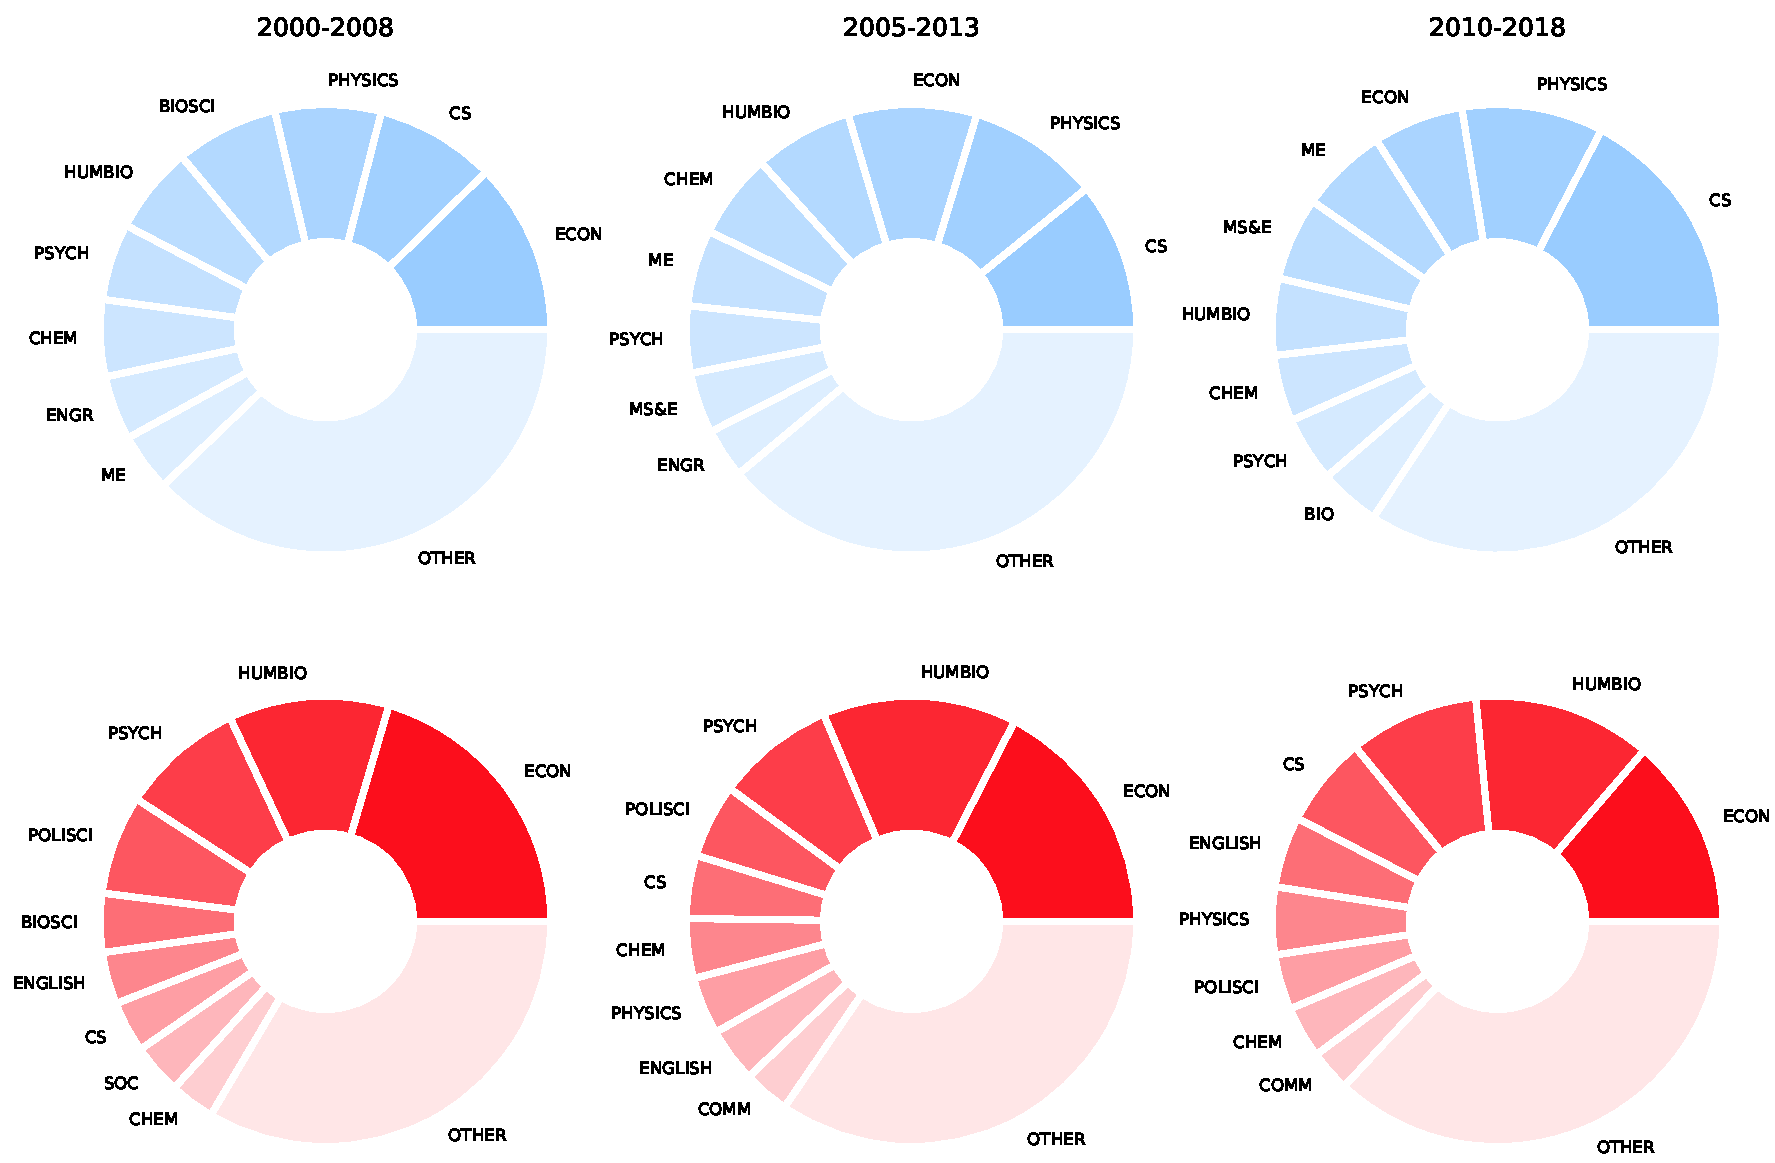
\includegraphics[width=\columnwidth]{final-evolution.pdf}
    \caption{A comparison over time of PageRank values by department in both the entire undergraduate network (light blue) and the undergraduate network filtered on students who earned a Bachelor's of Arts (BA) degree (red). We argue that PageRank offers us a highly flexible method of determining course accessibility based on aggregate student behavior.}
    \label{fig:evolution}
\end{figure}

For a given department with PageRank score $X$, starting at a random course and selecting successors at random will land you in this department $(X * 100)$\% of the time. We use strict counts of pairwise course sequences from quarter to quarter in order to define edge weights between courses, which are then used as transition probabilities during PageRank execution. From a graph theoretic perspective this approach signals connectedness of department courses to other courses in the graph.

More generally, we can interpret the relative size of the departments in the figure above as the accessibility of departments across the different disciplines at the university throughout any time period in an undergraduate's career. Indeed, one could interpret this as an inverse relationship with the activation energy required to begin taking courses in a given department. In this case a department's high PageRank score would indicate a relative ease of entering a particular department. While closely linked, this differs from metrics regarding course composition and university enrollment due to the emphasis on the flow of students from course to course. Paired with student demographic information, one could use PageRank in order determine the accessibility of courses and departments based on past student behavior.

We observe that between 2000 and 2018, the PageRank score of the Computer Science department has only increased. This applies in general to all degree-seeking students and to the BA-seeking students. Similarly we note a rise in the amount of Physics courses taken during this time window. It is unclear whether the increase enrollment in Physics classes is due to more interest in this department or if the popularity increase in Computer Science, which requires taking several Physics classes, has promoted this observed trend. Another point to note is a general decrease in enrollment of economics courses, but a noticeable uptick in the amount of classes taken in Management Sciences and Engineering (MS\&E). These two trends are strongly correlated, as the material of MS\&E seeks to combine economics and finance with computer science and statistics. 

Our results are more generally in support of observations made by education researchers. Over the past 20 years the proportion of students majoring in STEM, and particularly computer science has varied greatly \cite{ComputingResearchAssociation2017}. Introductory, mid-level and upper-level computer sciences courses have all shown a demonstrable increase upwards of 150\% of student enrollment between 2000 and 2017. Driving student's decisions to enroll in more technical courses is primarily the greater monetary compensation that these majors promise at the workplace \cite{Downey2007}. Interestingly, however, while the total amount of classes taken within Computer Science has risen noticeably, we do not observe that the total amount of student majors in Computer Science has increased at the same rate. Rather between 2000 and 2010 the number of Computer Science majors showed an uptick of only (INSERT NUMBER) percent. Stretching this time interval to between 2000 and 2018 this number increases to (INSERT NUMBER) percent. This finding is more generally in line with the observed trend that the Computer Science major has not experienced a constant exponential increase in popularity. Rather, 2005 was one of the years with the lowest rates of students who self-reported interest in majoring in Computer Science when entering college \cite{Patterson2005}. Between 2000 and 2008 it was, in fact, economics and business-related courses that remained one of the most popular majors of study nation wide \cite{NationalCenterforEducation2018}. Overall, our quantitative analysis is able to corroborate much of the education research regarding course enrollment patterns over the past 20 years. We stress that the methodology used to generate these results is not dependent on the source of data, but is rather facilitated by the graphical modeling of student course enrollments that \textit{Via} enables.

\subsection{Student Stakeholders}
\label{sec:student_stakeholders}
Among university stake-holders, students are one of the principal groups that would benefit from the clear insights that can be gleamed from the \textit{Via} toolkit. In this section we will highlight two particular use-cases. First, our visual modeling of course sequences allows a student to identify which majors require students to take courses from within only a certain department and which allow for more academic exploration across departments. We can report this result both visually, by directly looking at the inter-departments orange arrows in a graph, and by calculating the modularity of certain departments. Modularity is a metric that represents the connectivity of clusters within a graph, by calculating the over-representation of edges among group of nodes.

In figure \ref{fig:modularity}, we compare the interconnectivity of the History and Electric Engineering majors.  Observe that the rings come from a conditional probability projection model using a discrete discount function $d$ that only captured proximate course enrollments (one academic time-step apart). Here we see that the visualizations align with the modularity scores associated with History (0.003) and Electrical Engineering (0.028), as the higher the modularity score the more a department is interconnected.

\begin{figure}
    \centering
    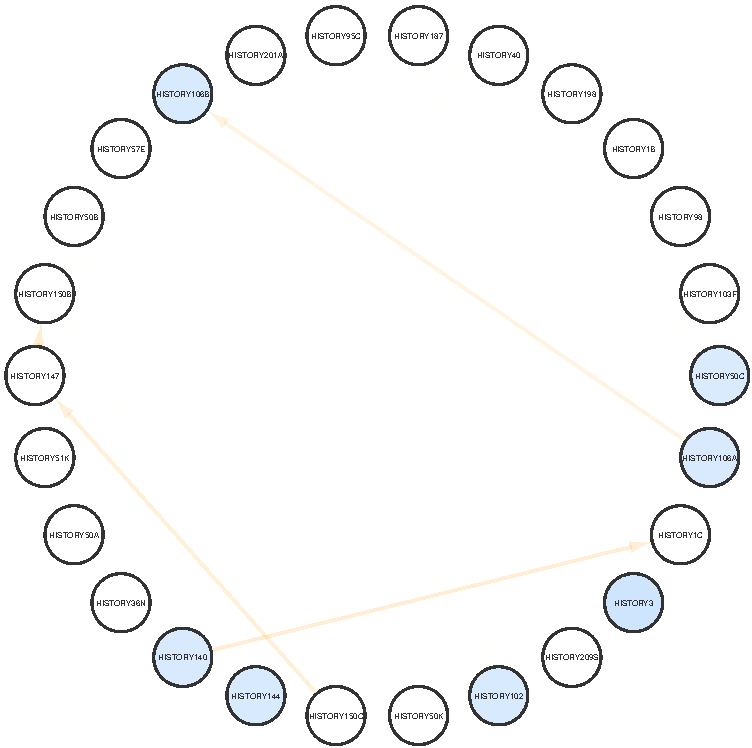
\includegraphics[width=0.55\columnwidth]{final-modularity-history.pdf}
    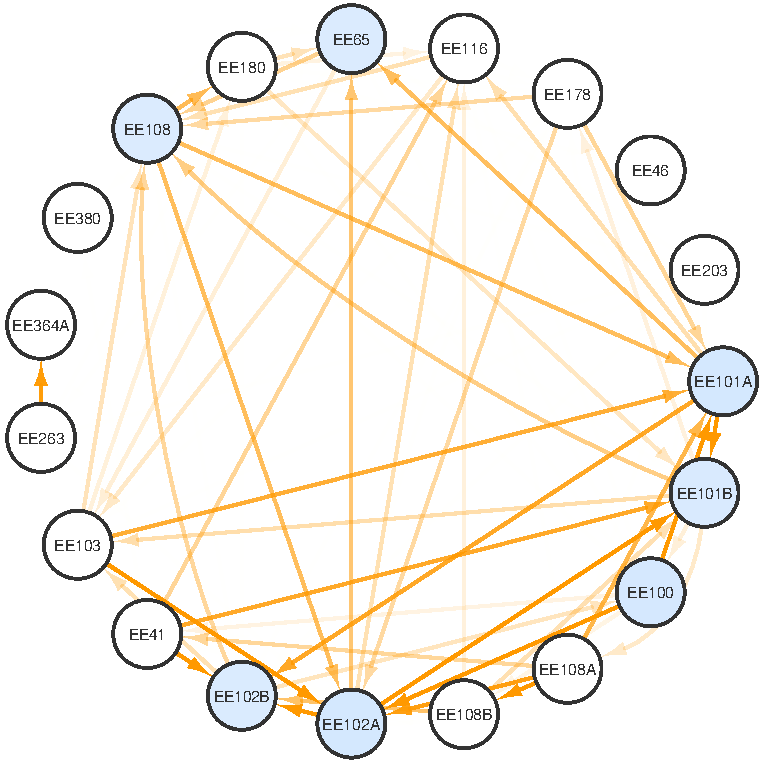
\includegraphics[width=0.44\columnwidth]{final-modularity-ee.pdf}
    \caption{A comparison between the student behavioral patterns in two departments--- History (left) and Electrical Engineering (right)--- from the years 2012-2016}
    \label{fig:modularity}
\end{figure}

As a second use-case we illustrate how \textit{Via} can be leveraged to discover the 'try-me' courses within department. That is to say, given that a student is currently majoring in a major x but interested in exploring other fields of study our model can recommend ideal courses to try in other departments. We find these 'try-me' courses by applying filtering on a particular major when creating the sequence model, and finding the most popular courses within this generated graph that are not in the major which we used as a filter. For instance by filtering on the history major, we observe that, of the History majors, nearly 28\% take CS105 and 21\% take CS106A. These are visualized through variations in node coloration in figure \ref{fig:history-try-me}.

\begin{figure}[h]
    \centering
    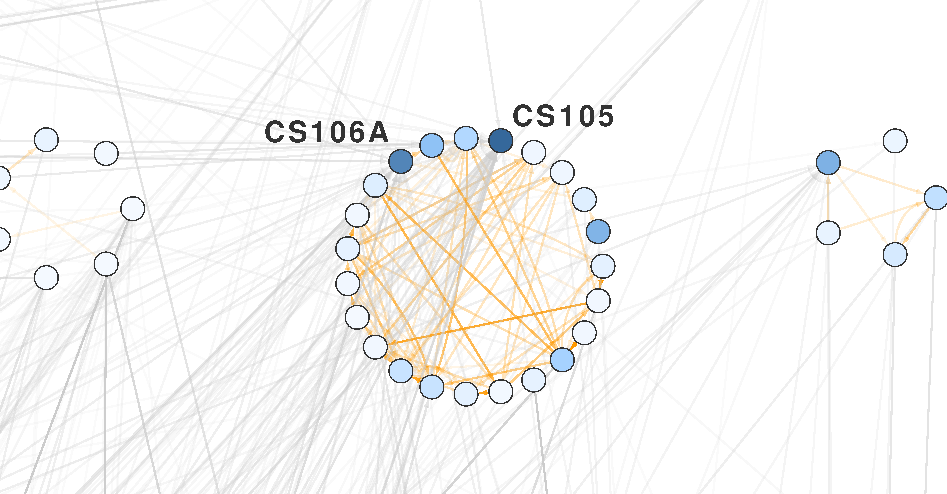
\includegraphics[width=.9\columnwidth]{final-history-try-me.pdf}
    \caption{Try-me courses in CS for History majors.}
    \label{fig:history-try-me}
\end{figure}

\subsection{Instructor Stakeholders}
\label{sec:instructor_stakeholders}

Instructors are a second group of stakeholders that can benefit from the easy interpretability of course sequence visualization. It is of particular interest to instructors to gain an overview of which sorts of students are enrolling in their courses. 

In figure (\ref{fig:spanlang}), we show that it is possible to use the course probabilities associated with course-to-course interactions in order to study the background of students who take higher-level Spanish language classes. We do this by simply examining the conditional probability graph generated with all enrollment data. We set our function $d$ as sensitive only to enrollments in course pairs within one year of each other in order to capture delayed enrollment behaviors. We can thus interpret edge weights as probability $p(i|j \text{ within the past year})$. Examine the courses associated with the V-structure colored in red--- \textsc{spanlang3} (bottom middle), \textsc{spanlang2a} (bottom right), and \textsc{spanlang11c} (top middle). \textsc{spanlang3} is the final quarter of the non-accelerated offering of the first-year Spanish language sequence, \textsc{spanlang2a} is the final quarter of the accelerated first-year sequence (often taken by students with prior exposure to the language through high school programs), and \textsc{spanlang11c} is the first quarter of the second-year sequence.

From the visualization alone, it is evident that the relationship between \textsc{spanlang3} and \textsc{spanlang11c} is stronger than the relationship between \textsc{spanlang2a} and \textsc{spanlang11c}. Indeed, the probability that a student enrolls in \textsc{spanlang11c} within a year of completing \textsc{spanlang3} is almost three times that of a student who enrolls in \textsc{spanlang11c} after completing \textsc{spanlang2a}, with $p(\textsc{spanlang11c}|\textsc{spanlang3}) = 0.038$ and $p(\textsc{spanlang11c}|\textsc{spanlang2a}) = 0.013$. It is possible that this stems from a difference in the instruction of a grammatical foundations between the university's introductory courses and high school language programs. If so, then this observation is in accordance with the research of Leaver \textit{et al.}, which details the significance in varying teaching philosophies commonly seen in foreign language classrooms at different language acquisition levels \cite{Leaver2002}.

While one may interpret this observation in many ways, we argue that the simplicity of the process through which this information can be found greatly decreases the time and effort required to observe enrollment patterns from the perspective of university administration.

\begin{figure}[h]
    \centering
    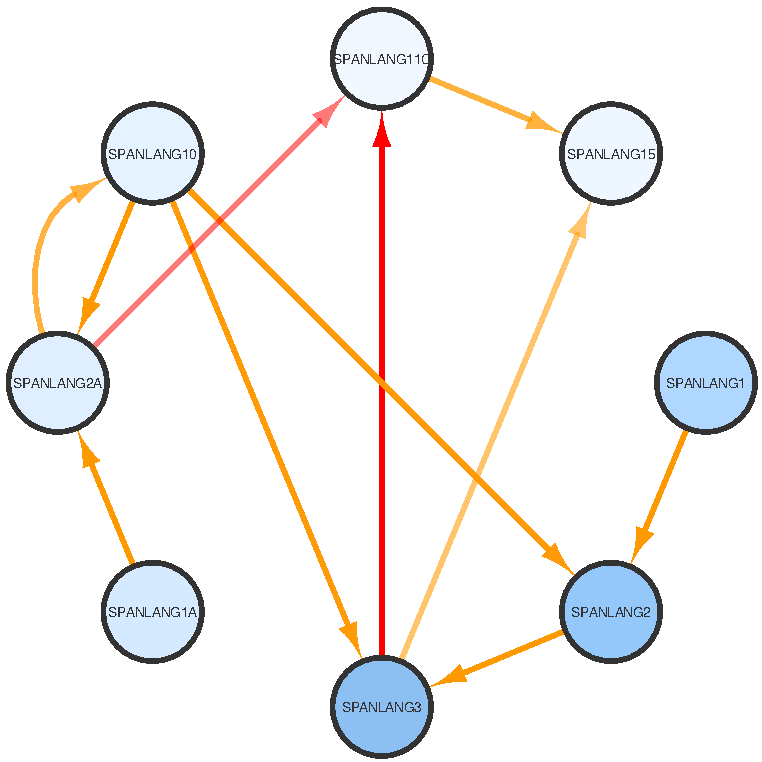
\includegraphics[width=\columnwidth]{final-spanlang.pdf}  
    \caption{Relationships within the language department's Spanish course offerings from 2012-2016, as projected by the conditional probability projection model using a discrete discount function $d$ that captures relationships between courses taken within one year of each other (Best viewed in color). We note that the probability that a student transitions from first to second year Spanish significantly increases if initially enrolled in the non-accelerated track.}
    \label{fig:spanlang}
\end{figure}

\subsection{Administrative Stakeholders}
\label{sec:administrative_stakeholders}

Finally, we believe that our model provides an intuitive medium for understanding department-wide dynamics across varying student demographics. Administrators in charge of course resource allocation may be interested in the enrollment patterns of students as they move through a department's course offerings. We provide two use-cases to illustrate how \textit{Via} can be used in order to derive insights about the structure of courses within department.

First, we study which classes within a department are the classes that tend to guide a student into a certain department. That is to say, we report the top 10 classes within a department that once taken by a student have the highest likelihood that a student continues taking classes within the same department. This 'persistence within a department' metric can be computed for a given class i in a department x by finding the number of expected courses that are taken within the department x after haven taken class i. In figure \ref{fig:persistence} we show the student persistence within a department using a raw count projection model with discrete discount function $d$ that captured all non-co-enrollment relationships between courses from 2014-2018. Here we measure the average number of courses taken within a department after having enrolled in a given course. Within the Biology (right) and Chemistry (middle) departments, we recover the insight that the 1-unit companion courses to the introductory courses (BIO41A and CHEM31AC for Biology and Chemistry, respectively) improved student persistence in that enrollment in these courses led to an overall increase in the number of courses taken within the department, on average. We contrast this with the Math department. Those who enrolled in the most courses offered within the Math department were those who enrolled in the first course of the honors multivariable mathematics sequence, MATH51H. 

\begin{figure*}[h!]
    \centering
    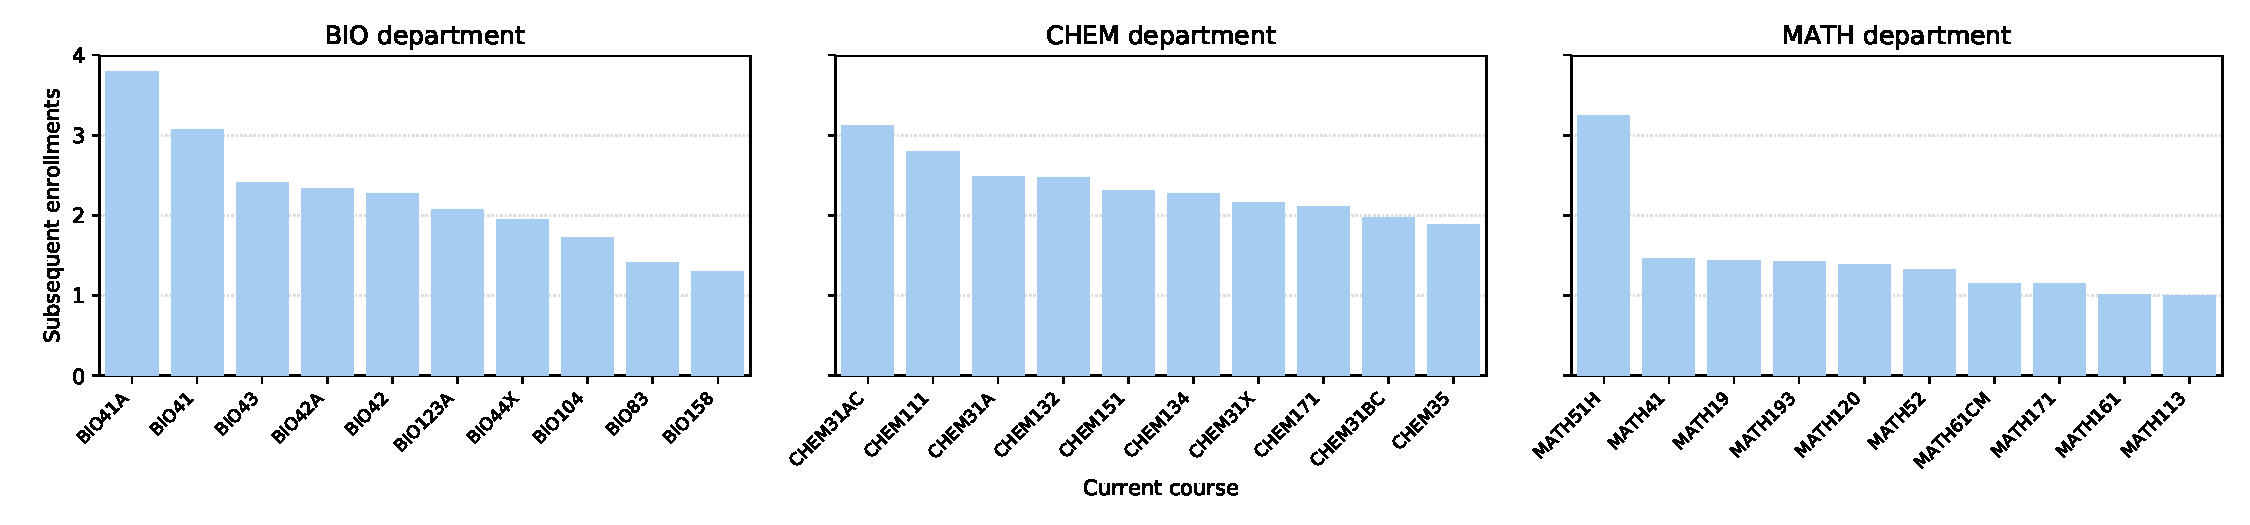
\includegraphics[width=18cm]{final-persistence.pdf}
    \caption{Student Persistence Metrics in Biology, Chemistry and Mathematics}
    \label{fig:persistence}
\end{figure*}

We also illustrate how we can recover particular 'roles' of courses in a certain department. The application of algorithms rooted in graph theory such as RolX \cite{Henderson2012} can allow third party researchers and other parties to recover fine-grained course dynamics from university enrollment data alone. This decreases greaty the onboarding time that is necessary in when becoming familiar with a new university's course offerings. In this example, we present the usage of RolX in order to discover the roles of courses as they pertain to students. We posit the successful recovery of introductory courses (red), intermediate courses (blue), and senior project / enrichment courses (green) due to the metrics recovered by NodeSense.


\begin{figure}
    \centering
    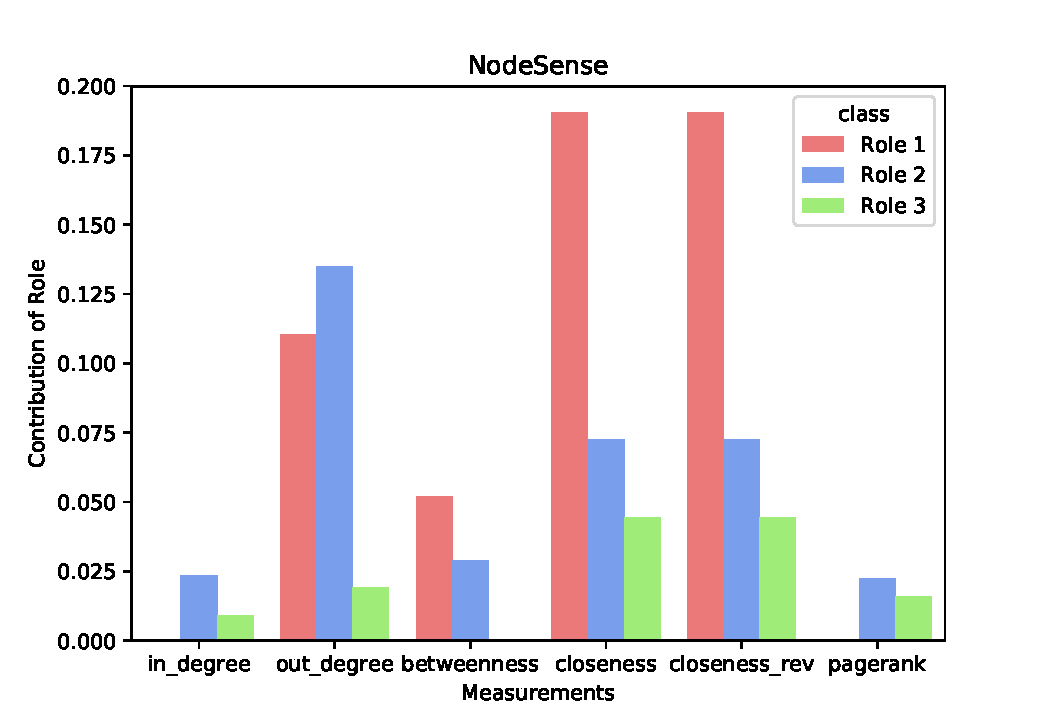
\includegraphics[width=0.75\columnwidth]{final-rolx-sense.pdf}
    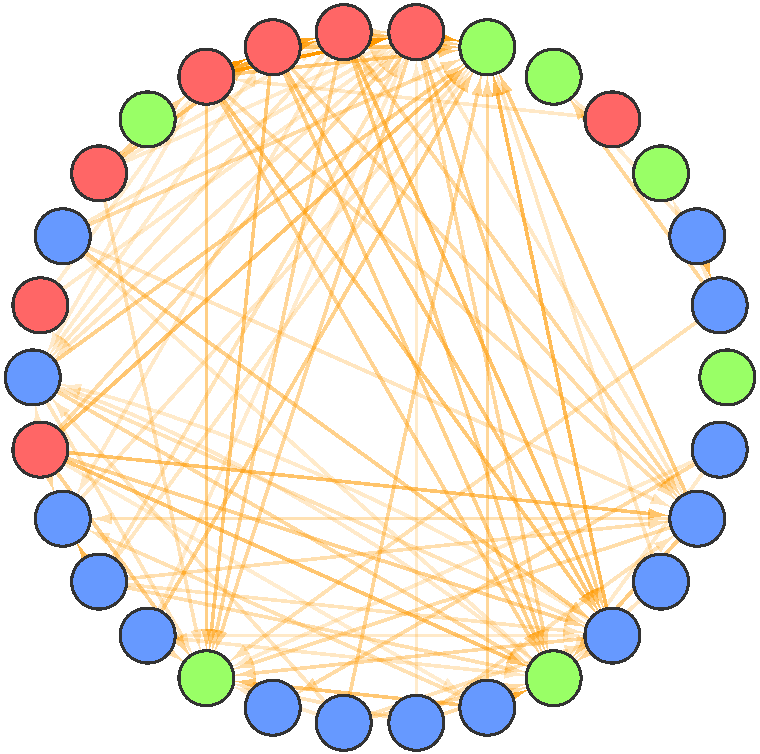
\includegraphics[width=0.24\columnwidth]{final-rolx.pdf}
    \caption{RolX Analysis of Course Sequences}
    \label{fig:rolx}
\end{figure}

%% \section{Other Applications}

\section{Conclusion and Future Work}
\label{sec:conclusion}
We have demonstrated a new approach to visualizing and interpreting transcript enrollment data available at every major American university. We've proposed a visualization toolkit that allows stakeholders such as students, advisors, and department chairs to understand aggregate student behavior over time. Using graph theoretic principles, we have presented several use cases for our projection model and in doing so have provided some insight into course trends at Stanford University.

We will be continuing experiments using this paradigm in order to better understand the effects of the demand increase in Computer Science at a university wide level. We have just scratched the surface in student behavior analysis. Future work includes running various feature representation algorithms such as node2vec and DeepWalk in order to visualize changes in course relationships over time. We will also be analyzing the results of running the PageRank algorithm on the various projection models made possible by our model in an attempt to better understand the similarities between courses.

% BALANCE COLUMNS
\balance{}
% REFERENCES FORMAT
% References must be the same font size as other body text.
\bibliographystyle{SIGCHI-Reference-Format}
\bibliography{coursePrecedence}

\end{document}

%%% Local Variables:
%%% mode: latex
%%% TeX-master: t
%%% End:
